\documentclass[a4paper, twocolumn]{article}
\usepackage[pdftex]{graphicx}                % Improved inclusion of .pdf-graphics files.
\usepackage{sidecap}                         % Floats with captions to the right/left.
\usepackage{enumerate}                       % Change counters (arabic, roman, etc.).
\usepackage{floatrow}                        % Multi-figure floats.
\usepackage{subfig}                          % Multi-figure floats.
\usepackage{bm}                              % Bolded text in math mode.
\usepackage[framemethod=default]{mdframed}   % Make boxes.
\usepackage{listings}                        % For including source code.
\usepackage{mathtools}                       % Underbrackets, overbrackets.
\usepackage[dvipsnames]{xcolor}              % Colors.
\usepackage{capt-of}                         % Caption things which are not floats.
\usepackage{fontawesome}                     % Github icon, etc. \faGithub
\usepackage{sidecap}                         % Floats with captions on the side.
\usepackage{tabularx}                        % Tables and stuff.
\usepackage{tabulary}                        % Tables and stuff.
\usepackage[sf,sl,outermarks]{titlesec}      % Change fonts in section{}, subsection{}, etc.
\usepackage[subfigure]{tocloft}              % Change spacing between numbers and titles in TOC.
\usepackage{booktabs}                        % \toprule, \midrule, etc. for tables.
\usepackage{siunitx}                         % Allows S table column, aligning on decimal point.
\usepackage{chngcntr}                        % Change counter behaviour, supress increment of sub counters.
\usepackage[%                                % Adds functionality to captions.
tableposition = top,
labelsep      = period,
justification = raggedright,
format        = hang,
]{caption}
\usepackage[%                                % Interactive references and links, colored.
colorlinks  = true,
linkcolor   = black,
urlcolor    = blue,
citecolor   = black,
linktocpage = true,
]{hyperref}
\usepackage[%                                % References, in super-script form.
autocite    = superscript,
backend     = biber,
sortcites   = true,
style       = numeric-comp,
sorting     = none,
url         = false,
]{biblatex}
\usepackage[autostyle, english = american]{csquotes} % Assure quotation marks are inserted correctly aligned left/right.
\MakeOuterQuote{"}

% Package settings ----------------------------------------------------------- %
%\renewcommand{\thesection}{\Roman{section}}         % I, II, III, IV, etc. section numbering
%\renewcommand{\thesubsection}{\Alph{subsection}}    % A, B, C, etc. subsection numbering
\renewcommand{\thesubsubsection}{}                  % Remove subsubsection numbering.
\floatsetup[table]{capposition=top}                 % Place table captions above the table.
\captionsetup[subfigure]{labelformat=empty}         % Remove the (a), (b), etc. tags from subfigures.
\advance\cftsecnumwidth 1.0em\relax                 % Set the spacing between section headings and titles in TOC with tocloft.
\advance\cftsubsecindent 1.0em\relax                % Set the spacing between subsection headings and titles in TOC with tocloft.
\advance\cftsubsecnumwidth 1.0em\relax              % Set the spacing between subsubsection headings and titles in TOC with tocloft.
\newcommand{\listingsfont}{\ttfamily}
\newcommand{\inlinepy}[1]{\lstinline[language={python}]{#1}}
\newcommand{\inlinecc}[1]{\lstinline[language={c++}]{#1}}
\counterwithout*{subsection}{section}               % Dont reset the subsection counter on new \section{} calls.
\renewcommand{\figurename}{FIG.}                    % Captions of figures read FIG.
\renewcommand{\tablename}{TABLE}                    % Captions of tables read TABLE
\renewcommand{\thetable}{\Roman{table}}             % Number tables with roman numerals.

% Section headings settings -------------------------------------------------- %
\titleformat{\section}[hang]  % {command}[shape]
{\normalfont\bfseries}      % {format}
{\thesection.}              % {label}
{2ex}                       % {sep}
{\centering\MakeUppercase}  % {before-code}[after-code]

\titleformat{\subsection}[hang] % {command}[shape]
{\normalfont\bfseries}        % {format}
{\thesubsection.}             % {label}
{1ex}                         % {sep}
{\centering}                  % {before-code}[after-code]

\titleformat{\subsubsection}[hang]  % {command}[shape]
{\normalfont\bfseries}            % {format}
{}                                % {label}
{1ex}                             % {sep}
{\centering}                      % {before-code}[after-code]


% References ----------------------------------------------------------------- %
\newcommand{\Fig}[1]{Fig.\ \ref{fig:#1}}
\newcommand{\fig}[1]{Fig.\ \ref{fig:#1}}
\newcommand{\eq} [1]{Eq.\ (\ref{eq:#1})}
\newcommand{\Eq} [1]{Eq.\ (\ref{eq:#1})}
\newcommand{\tab}[1]{Table \ref{tab:#1}}
\newcommand{\Tab}[1]{Table \ref{tab:#1}}

% Matrices ------------------------------------------------------------------- %
\newcommand{\mat} [2]{\begin{matrix}[#1] #2 \end{matrix}}    % Nothing enclosing it.
\newcommand{\pmat}[2]{\begin{pmatrix}[#1] #2 \end{pmatrix}}  % Enclosing parentheses.
\newcommand{\bmat}[2]{\begin{bmatrix}[#1] #2 \end{bmatrix}}  % Enclosing square brackets.
\newcommand{\vmat}[2]{\begin{vmatrix}[#1] #2 \end{vmatrix}}  % Enclosing vertical bars.
\newcommand{\Vmat}[2]{\begin{Vmatrix}[#1] #2 \end{Vmatrix}}  % Enclosing double bars.

% Manually set alignment of rows / columns in matrices (mat, pmat, etc.) ----- %
\makeatletter
\renewcommand*\env@matrix[1][*\c@MaxMatrixCols c]{%
  \hskip -\arraycolsep
  \let\@ifnextchar\new@ifnextchar
  \array{#1}}
\makeatother

% figures in multicols environment ------------------------------------------- %
\newenvironment{Figure}
{\par\medskip\noindent\minipage{\linewidth}}
{\endminipage\par\medskip}

% Set bibliography file and path for images.
\addbibresource{../ref/project1-references.bib}
\bibliography{../ref/project1-references.bib}
\graphicspath{{../figs/}}

% Black frame with gray background ------------------------------------------ %
\definecolor{gray}{gray}{0.9}
\newmdenv[linecolor=white,backgroundcolor=gray]{grayframe}

% Title
\title{{\sc Regression and Resampling methods \\ {\large FYS-STK4155: Project 1}}}
\author{Trygve Leithe Svalheim \\ \faGithub \ {\small \href{https://github.com/trygvels/FYS-STK4155}{github.com/trygvels/FYS-STK4155}}}
  

\begin{document}


\twocolumn[
\begin{@twocolumnfalse}
\maketitle
\begin{abstract}
\end{abstract}

\tableofcontents 
\end{@twocolumnfalse}]
\clearpage
%\newpage



\iffalse
\section{Figurestuff}
Interesting figures:
Fit to franke function for OLS for different noise 3x
Ridge with different lambdas 4x
Lasso for different lambdas 4x
BV OLS
BV ridge for optimal lamb?
BV lasso for optimal lamb?

Beta verdier per lambda for lasso og ridge

Terrain data analyse ??

kanskje error per noise

subsection{Datanotes}

OLS

Noise = 0
Polynomial of degree:  5
Total error on training data:
MSE: 0.00227,  R^2: 0.97209
Total error on test data:
MSE: 0.00297,  R^2: 0.96355
Too few polynomial degrees for bias-variance plot

N = 0.01
Polynomial of degree:  5
Total error on training data:
MSE: 0.00230,  R^2: 0.97188
Total error on test data:
MSE: 0.00299,  R^2: 0.96351
Too few polynomial degrees for bias-variance plot

N = 0.05
Polynomial of degree:  5
Total error on training data:
MSE: 0.00431,  R^2: 0.94976
Total error on test data:
MSE: 0.00528,  R^2: 0.93844
Too few polynomial degrees for bias-variance plot


Noise = 0.1
Polynomial of degree:  5
Total error on training data:
MSE: 0.01106,  R^2: 0.88366
Total error on test data:
MSE: 0.01312,  R^2: 0.86203
Too few polynomial degrees for bias-variance plot

Ridge N0.1

Polynomial of degree:  5
Total error on training data:
MSE: 0.01171,  R^2: 0.87685
Total error on test data:
MSE: 0.01333,  R^2: 0.85982
Too few polynomial degrees for bias-variance plot

Polynomial of degree:  5
Total error on training data:
MSE: 0.01333,  R^2: 0.85978
Total error on test data:
MSE: 0.01451,  R^2: 0.84744
Too few polynomial degrees for bias-variance plot

Polynomial of degree:  5
Total error on training data:
MSE: 0.01563,  R^2: 0.83561
Total error on test data:
MSE: 0.01728,  R^2: 0.81822
Too few polynomial degrees for bias-variance plot

Polynomial of degree:  5
Total error on training data:
MSE: 0.01832,  R^2: 0.80738
Total error on test data:
MSE: 0.01940,  R^2: 0.79600
Too few polynomial degrees for bias-variance plot

Polynomial of degree:  5
Total error on training data:
MSE: 0.02000,  R^2: 0.78971
Total error on test data:
MSE: 0.02075,  R^2: 0.78173
Too few polynomial degrees for bias-variance plot


LASSO

Polynomial of degree:  5
Total error on training data:
MSE: 0.01722,  R^2: 0.81885
Total error on test data:
MSE: 0.01856,  R^2: 0.80476
Too few polynomial degrees for bias-variance plot

Polynomial of degree:  5
Total error on training data:
MSE: 0.02135,  R^2: 0.77550
Total error on test data:
MSE: 0.02176,  R^2: 0.77116
Too few polynomial degrees for bias-variance plot

Polynomial of degree:  5
Total error on training data:
MSE: 0.03412,  R^2: 0.64119
Total error on test data:
MSE: 0.03568,  R^2: 0.62481
Too few polynomial degrees for bias-variance plot

Polynomial of degree:  5
Total error on training data:
MSE: 0.09506,  R^2: 0.00023
Total error on test data:
MSE: 0.09529,  R^2: -0.00210
Too few polynomial degrees for bias-variance plot

Polynomial of degree:  5
Total error on training data:
MSE: 0.09507,  R^2: 0.00022
Total error on test data:
MSE: 0.09527,  R^2: -0.00196
Too few polynomial degrees for bias-variance plot
\fi
%%-----------------
%% INTRODUCTION
\section{Introduction}

In this project we explore the problem of regression analysis, resampling and optimal hyperparemeters. Regression is the process modelling a response $y$ through the parameterization of a predictor variable $x$ ???. This is a powerful tool, as it gives us the ability to minimize the difference between observed data $y$ and predicted data $\tilde{y}$ and solve for an optimal predictor. In this work, our focus will be on Linear regression, where the relationship between $x$ and $y$ is strictly linear and can be described by the model
\begin{equation}
  \mathbf{\tilde{y}} = \mathbf{X}\mathbf{\beta},
\end{equation}
and the true responsecan be described with the addition of an error term $\epsilon$, denoting the modelling error so that
\begin{equation}
  \mathbf{y} = \mathbf{X}\mathbf{\beta}+\mathbf{\epsilon}.
\end{equation}
Linear regression is a fundamental method of statistical analysis, and allows us to study the relationships hidden in all types of data sets, which is increasingly powerful in a world where data is both abundant and complex.
In this study, we look at three common regression methods and assess their capabilities on two different data sets. In addition, we explore the importance resampling methods and the impact of hyperparemeters and their data dependence.

%% -----------------
\section{Regression methods}
In this section we outline the basics of three different regression methods which we later apply to our two data sets. 
\subsection{Ordinary Least Squares (OLS)}
As briefly mentioned in the introduction, a Linear regression system revolves around modeling a function $\mathbf{y}\mathbf{X}$, where the matrix $\mathbf{X}$ containing the predictors is called \textit{design matrix}. Again, we want to find the values of $\beta$, that minimizes the error $\epsilon$ describing the difference between the predicted and true values $\mathbf{\tilde{y}}$ and $\mathbf{y}$.
However, there are several different ways of describing the error, for the first method, the \textit{Ordinary Least Squares (OLS)} method, we chose a \textit{cost function} parameterized by the Euclidean $L^2$ norm,
\begin{align}
C(\bm\beta) &= \Vert \mathbf{y} - \tilde{\mathbf{y}}\Vert_2^2 \nonumber \\
&= \sum_{i=1}^n \Big| y_i - \sum_{j=0}^p X_{ip} \beta_p \Big|^2. \label{eq:cost}
\end{align}
Furthermore we can quantize the full error using the \textit{Mean Squared Error} (MSE), which is simply the ensamble average over the $L^2$-loss.
For this particular error metric, the optimal $\beta$ parameters can be found by minimising this function.
The linear algebra representation of this minimization problem can be described by

\begin{align}
\frac{\partial C(\bm\beta)}{\partial \bm\beta} &= \frac{\partial}{\partial \bm\beta} (\mathbf{y}-\mathbf{X}\bm\beta)^T (\mathbf{y}-\mathbf{X}\bm\beta) = 0 \nonumber \\
\bm\beta_\text{optimal} &= \left(\mathbf{X}^T\mathbf{X}\right)^{-1}\mathbf{X}^T\mathbf{y}.
\end{align}
For some datasets, the inversion operation $\left(\mathbf{X}^T\mathbf{X}\right)$ is too costly. With the data sizes we are dealing with this should, not lead to any problems. However, in order to generalize our program, we chose to employ the Singular Value Decomposition (SVD) method. Without going into the details of the method, it works by decomposing the matrix $X$ into more computationally tractable matrixes;
\begin{align}
\mathbf{X} = \mathbf{U}\mathbf{\Sigma}\mathbf{V}^T.
\end{align}
Using this definition, it can be shown that
\begin{align}
\tilde{\mathbf{y}}_\text{OLS} &= \mathbf{X}\bm\beta_\text{OLS} \nonumber \\
&= \mathbf{X}\left(\mathbf{X}^T\mathbf{X}\right)^{-1}\mathbf{X}^T\mathbf{y} \nonumber \\
&= \mathbf{X} \left[ \left(\mathbf{U}\bm\Sigma \mathbf{V}^T\right)^T \mathbf{U}\bm\Sigma \mathbf{V}^T \right]^{-1} \mathbf{X}^T \mathbf{y} \nonumber \\
&= \mathbf{U}\mathbf{U}^T\mathbf{y}. \label{eq:principal1}
\end{align}
The OLS method is thus a simple and straight forward method which is surprisingly powerful even without a regularization term, which is the key difference between it and Ridge regression.

\subsection{Ridge regression}
A common problem in regression and machine learning is overfitting. When the complexity of the model increases, the system tries too hard to fit the training data, ultimately increasing the error on the test data. Ridge regression attempts to combat this, by introducing an alternative cost function
\begin{align}
  C(\boldsymbol{X},\boldsymbol{\beta})=\frac{1}{n}\vert\vert \boldsymbol{y}-\boldsymbol{X}\boldsymbol{\beta}\vert\vert_2^2+\lambda\vert\vert \boldsymbol{\beta}\vert\vert_2^2.
\end{align}
With the addition of a regularization term, quantized by the hyperparameter $\lambda$, we penalize high values of $\beta$. This effectively simplifies the solution, making the model less flexible, reducing the variance. The drawback, however, is that this also increases the bias 

which penalizes high values of $\beta$ according to the hyperparamter   counteracting the effect of overfitting. As we will later discuss, when increasing the complexity of our model, our system becomes increasingly susceptible to overfitting the training data. With the implementation of the regularization term, we force the system to converge on a ``simple'' model, effectively reducing the variance. 

\subsection{Lasso regression}
The last of the trio is Lasso regression. It is similar to Ridge in the way that it adds a regularization term, but more aggressively so. This becomes evident when we once again look at the cost function
\begin{align}
  C(\boldsymbol{X},\boldsymbol{\beta})=\frac{1}{n}\vert\vert \boldsymbol{y}-\boldsymbol{X}\boldsymbol{\beta}\vert\vert_2^2+\lambda\vert\vert \boldsymbol{\beta}\vert\vert_1.
\end{align}
Here, the regularization comes on the form of $L^1$, which forces $\beta$-values to zero for sufficiently large values of $\lambda$.


\section{Data}
In this project we have tested the three previously discussed regression methods on two different data sets. First, we fit a polynomial to the \textit{Franke function}, a common test function for such analyses. Last, we assess our polynomial regression fits on real world terrain data.
\subsection{The Franke Function}
The Franke function is a two dimensional function developed to test interpolation techniques. However, its geometric features are well suited for our surface regression analysis as well. Mathematically, the Franke function is expressed as
\begin{align}
f_\text{F}(x,y) &= \frac{3}{4}\exp\left\{\frac{-1}{4}\left[\left(9x-2\right)^2 + \left(9y-2\right)^2\right]\right\}\nonumber \\
&+ \frac{3}{4}\exp\left\{\frac{-1}{49}\left(9x+1\right)^2 + \frac{1}{10}\left(9y+1\right)^2\right\}\nonumber \\
&+ \frac{1}{2}\exp\left\{\frac{-1}{4}\left[\left(9x-7\right)^2 + \left(9y-3\right)^2\right]\right\}\nonumber \\
&- \frac{1}{5}\exp\left\{\frac{-1}{4}\left[\left(9x+4\right)^2 + \left(9y-7\right)^2\right]\right\}.
\end{align}
A surface plot of the Franke function can be seen in figure \ref{fig:franke} evaluated over $x,y \in [0,1]$. 

\subsection{Terrain data}
The other data set employed in this study is taken from the U.S. Department of the Interior Geolocial Surveys (USGS) EarthExokirer website. The data is gathered from a Shuttle Radar Topography Mission (SRTM), which . More specifically, the area of land we are using is that of M\o svatn in Telemark. 


\section{Resampling and Bias variance}
Flexible models have higher variance, because they tend to overfit. 

\section{Application to real data}

%% -----------------
%% RESULTS
\section{Comparison}
Fitting to the Franke function



\begin{figure}
\centering
\includegraphics[width=\linewidth]{{BV_OLS_L0_franke_N0.1}.png}
\caption{Stuff}
\label{fig:distribution}
\end{figure}
      
\begin{figure}
\centering
\includegraphics[width=\linewidth]{{BV_ridge_L0.0001_franke_N0.1}.png}
\caption{Stuff}
\label{fig:distribution}
\end{figure}
      
\begin{figure}
  \centering
  \includegraphics[width=\linewidth]{{BV_lasso_L0.0001_franke_N0.1}.png}
  \caption{Stuff}
  \label{fig:distribution}
\end{figure}

\begin{figure*}[p]
\centering
\subfloat[$p=2$]{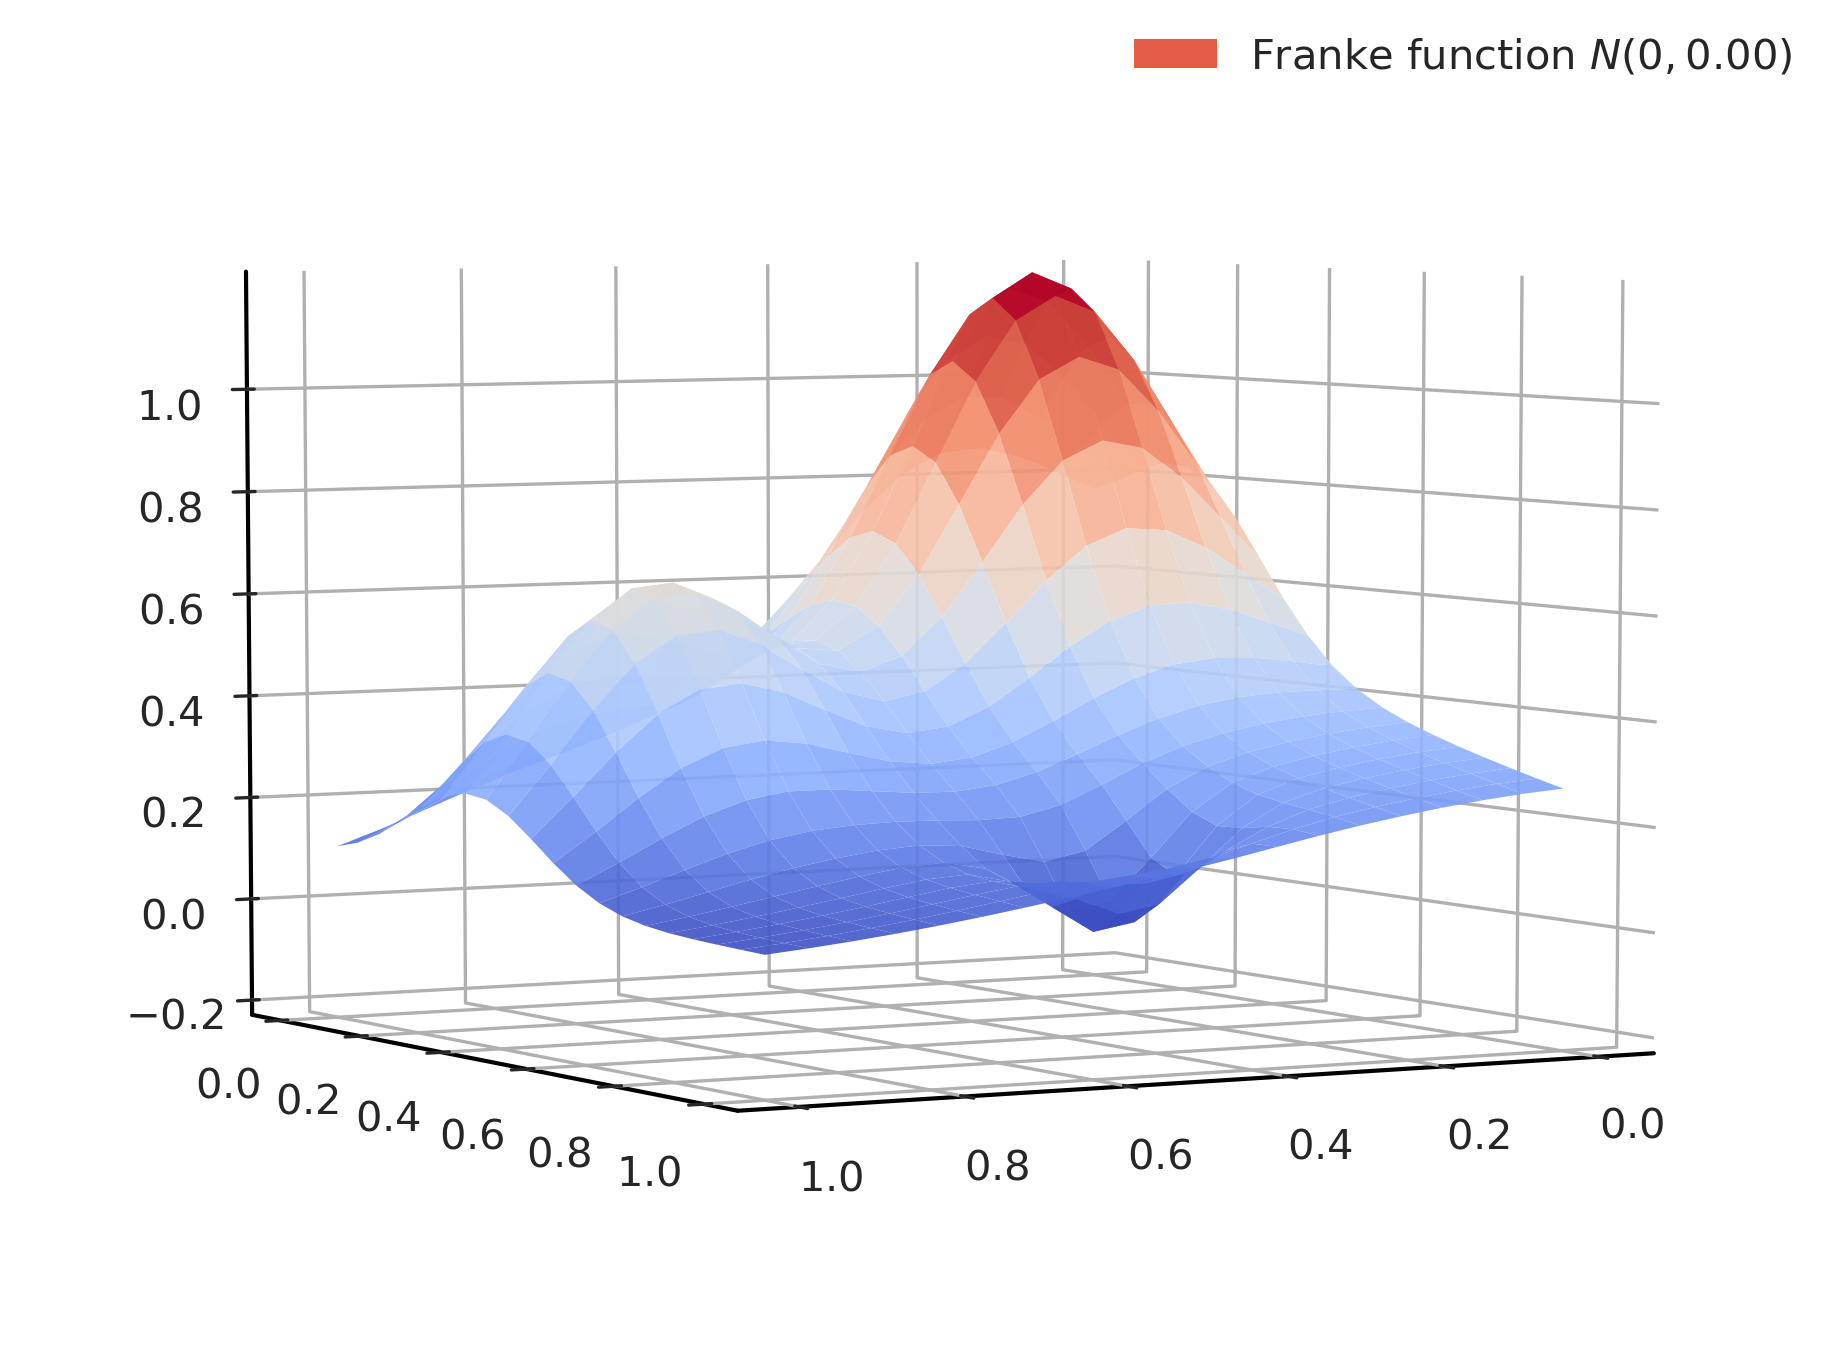
\includegraphics[width=0.48\linewidth]{franke.png}}
\subfloat[$p=3$]{\includegraphics[width=0.48\linewidth]{{OLS_L0_P5_franke_N0.05}.png}} \\[-20pt]
\subfloat[$p=4$]{\includegraphics[width=0.48\linewidth]{{OLS_L0_P5_franke_N0.1}.png}}
\subfloat[$p=5$]{\includegraphics[width=0.48\linewidth]{{OLS_L0_P5_franke_N0}.png}}
\captionof{figure}{OLS Regression. \label{fig:4}}
\end{figure*}


\begin{figure*}[p]
\centering
\subfloat[$\lambda=0.1$]{\includegraphics[width=0.48\linewidth]{{ridge_L0.1_P5_franke_N0.05}.png}} 
\subfloat[$\lambda=0.01$]{\includegraphics[width=0.48\linewidth]{{ridge_L0.01_P5_franke_N0.05}.png}}\\[-20pt]
\subfloat[$\lambda=0.001$]{\includegraphics[width=0.48\linewidth]{{ridge_L0.001_P5_franke_N0.05}.png}}
\subfloat[$\lambda=0.0001$]{\includegraphics[width=0.48\linewidth]{{ridge_L0.0001_P5_franke_N0.05}.png}}
\captionof{figure}{Ridge Regression. \label{fig:4}}
\end{figure*}

\begin{figure*}[p]
\centering
\subfloat[$\lambda=0.1$]{\includegraphics[width=0.48\linewidth]{{lasso_L0.1_P5_franke_N0.05}.png}} 
\subfloat[$\lambda=0.01$]{\includegraphics[width=0.48\linewidth]{{lasso_L0.01_P5_franke_N0.05}.png}}\\[-20pt]
\subfloat[$\lambda=0.001$]{\includegraphics[width=0.48\linewidth]{{lasso_L0.001_P5_franke_N0.05}.png}}
\subfloat[$\lambda=0.0001$]{\includegraphics[width=0.48\linewidth]{{lasso_L0.0001_P5_franke_N0.05}.png}}
\captionof{figure}{Lasso Regression. \label{fig:4}}
\end{figure*}


\begin{figure*}[p]
\centering
\subfloat[Ridge]{\includegraphics[width=0.48\linewidth]{{ridge_lambdas}.png}} 
\subfloat[Lasso]{\includegraphics[width=0.48\linewidth]{{lasso_lambdas}.png}}
\captionof{figure}{Values for $\beta$ for different values of the shrinkage parameter $\lambda$ using Ridge and LASSO regression. Confidence per parameter is calculated across all K-Folds, error bars 1 $\sigma$ confidence. \label{fig:4}}
\end{figure*}

%% ----------------
%% DISCUSSION
\section{Discussion}
		
%% ---------------
%% CONCLUSION
\section{Summary Remarks}
%\end{multicols}
\onecolumn{
\printbibliography
}
\end{document}
